\documentclass[11pt]{article}
\usepackage{amsmath, amssymb, amsthm}
\usepackage[retainorgcmds]{IEEEtrantools}

\usepackage{tikz}

\usepackage{fancyhdr}

%Format stuff
\pagestyle{fancy}
\headheight 35pt

%Header info
\chead{\Large \textbf{Loaded String}}
\lhead{}
\rhead{}

\begin{document}
The loaded string is fundamentally equivalent to an n-oscillator system, but normal modes are much easier to visualize when masses are displaced vertically in this system.
\begin{center}
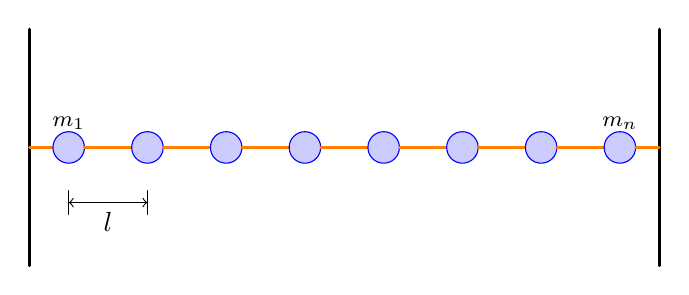
\begin{tikzpicture}
	[scale=1,line cap=round,
	%Styles
	axes/.style=,
	important line/.style={very thick},
	information text/.style={rounded corners,fill=red!10,inner sep=1ex},
	dot/.style={circle,inner sep=1pt,fill,label={#1},name=#1}			
	]
	
	%Colors
	\colorlet{anglecolor}{green!50!black}	%angle arcs/lines
	
	%The graphic
	\draw[color=black,very thick] (0, -1.5) -- (0, 1.5);
	\draw[color=black,very thick] (8, -1.5) -- (8, 1.5);
	\foreach \i in {.5,1.5,...,7.5}
	{
		\draw[color=orange,thick] (\i - .2, 0) -- +(-.3, 0);
		\filldraw[color=blue!20,draw=blue] (\i, 0) circle (.2);
		\draw[color=orange,thick] (\i + .2, 0) -- +(.3,0);
	}
	
	\node[above=3pt,black,font=\footnotesize] at (.5, 0) {$m_1$};
	\node[above=3pt,black,font=\footnotesize] at (7.5,0) {$m_n$};
	
	\draw (.5, -.55) -- (.5, -.85);
	\draw (1.5, -.55) -- (1.5, -.85);
	\draw[<->] (.5, -.7) -- node[below] {$l$} (1.5, -.7);
\end{tikzpicture}
\end{center}

If each mass in the system is displaced vertically a random amount, the free-body diagram for an arbitrary mass $m_p$ in the system looks like:
	\begin{center}
	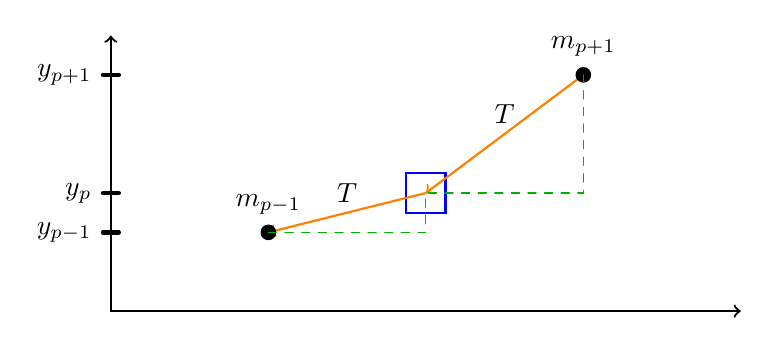
\begin{tikzpicture}
		[scale=1,line cap=round,
		%Styles
		axes/.style=,
		important line/.style={very thick},
		information text/.style={rounded corners,fill=red!10,inner sep=1ex},
		dot/.style={circle,inner sep=2pt,fill,label={#1},name=#1}			
		]
		
		%Colors
		\colorlet{anglecolor}{green!50!black}	%angle arcs/lines
		
		%The graphic
		\draw[thick,->] (0,0) -- (0, 3.5);
		\draw[thick,->] (0,0) -- (8, 0);
		
		\draw[blue,thick] (3.75, 1.25) rectangle (4.25, 1.75);
		\draw[<-,thick,orange] (4, 1.5) -- node[above,black] {$T$} (6, 3);
		\draw[->,thick,orange] (4, 1.5) -- node[above,black] {$T$} (2, 1);
		
		\node[dot=$m_{p+1}$] at (6, 3) {};
		\node[dot=$m_{p-1}$] at (2, 1) {};
		
		\draw[dashed,green!70!black] (2, 1) -- (4, 1) -- (4, 1.5) -- (6, 1.5) -- (6, 3);
		\draw[ultra thick] (-.1, 1) node[left] {$y_{p-1}$} -- (.1, 1);
		\draw[ultra thick] (-.1, 1.5) node[left] {$y_p$} -- (.1, 1.5);
		\draw[ultra thick] (-.1, 3) node[left] {$y_{p+1}$} -- (.1, 3);
	\end{tikzpicture}
	\end{center}
	
\section{Equation of Motion}
	\begin{equation}
		F_{y}^{(p)} = -T\sin(\alpha_{p-1}) + T\sin(\alpha_{p+1})
	\end{equation}
	Assuming small oscillations simplifies the calculation quite a bit.
	\begin{IEEEeqnarray}{rCl}
		\sin(\alpha_{p-1}) & \approx & \frac{y_p - y_{p-1}}{l}\\
		\sin(\alpha_{p+1}) & \approx & \frac{y_{p+1} - y_p}{l}
	\end{IEEEeqnarray}
	\begin{IEEEeqnarray}{rCl}
		-\frac{T}{l} (y_p - y_{p-1}) + \frac{T}{l}(y_{p+1} - y_p) & = & m\ddot{y}_p\\
		\ddot{y}_p + \frac{T}{ml}(2y_p) - \frac{T}{ml}y_{p-1} - \frac{T}{ml}y_{p+1} & = & 0
	\end{IEEEeqnarray}
	For the loaded string, set the natural frequency
	\begin{equation}
		\omega_0^2 = \frac{T}{ml}
	\end{equation}
	Which gives
	\begin{equation}
		\ddot{y}_p + 2\omega_0^2 y_p - \omega_0^2 (y_{p+1} + y_{p-1}) = 0
	\end{equation}
	
\section{Normal Modes}
	Making the assumption that the normal modes are in the form 
	\begin{equation}
		y_p = A_p e^{i\omega t}
	\end{equation}
	after substitution the following set of solutions is obtained.
	\begin{IEEEeqnarray}{rCl}
		y_p & = & c\sin(p\theta)e^{i\omega_p t}\\
		\omega_n & = & 2\omega_0 \sin\left(\frac{\theta}{2}\right)\\
		\theta & = & \frac{n\pi}{N+1}
	\end{IEEEeqnarray}
	
	Also, the relationship between adjacent amplitudes is
	\begin{equation}
		\frac{A_{p-1} + A_{p+1}}{A_p} = \frac{-\omega^2 + 2\omega_0^2}{\omega_0^2}
	\end{equation}
	
	In this equation, $p$ is an integer pointing to one of the masses in the system, and $N$ is the total number of masses. $n$ denotes which normal mode that the equation describes. There are $N$ different total normal modes in the system because the time evolution and amplitude are both periodic functions.
	
\section{General Solution}
	Just like the general solution to the coupled mechanical oscillators, the position of any one particle is a combination of normal modes.
	\begin{equation}
		y_p = \sum_{n=1}^N c_n \sin\left(\frac{n\pi}{N+1}\right) e^{i\omega_n t}
	\end{equation}
	Define the eigenvectors of each normal mode as
	\begin{equation}
		\mathbf{q_n} = \left( \sin \left(\frac{n\pi}{N+1}\right), \sin \left(\frac{2n\pi}{N+1}\right), \ldots , \sin \left(\frac{Nn\pi}{N+1}\right) \right)
	\end{equation}
	This gives the general solution to all the masses:
	\begin{equation}
		\mathbf{y} = \sum_{n=1}^N a_n \mathbf{q_n} e^{i\omega_n t}
	\end{equation}
%	\begin{center}
%	\begin{tikzpicture}
%		[scale=3,line cap=round,
%		%Styles
%		axes/.style=,
%		important line/.style={very thick},
%		information text/.style={rounded corners,fill=red!10,inner sep=1ex},
%		dot/.style={circle,inner sep=1pt,fill,label={#1},name=#1}			
%		]
%		
%		%Colors
%		\colorlet{anglecolor}{green!50!black}	%angle arcs/lines
%		
%		%The graphic
%	\end{tikzpicture}
%	\end{center}

%	\begin{figure}[htb]
%		\centering
%		\includegraphics[width=0.8\textwidth]{filename.eps}
%		\caption{Caption.}
%		\label{fig:figure}
%	\end{figure}

%		\def\enotesize{\normalsize}
%		\theendnotes
\end{document}